\documentclass[
    12pt,
    a4paper,
    sfdefaults=false,
    toc=chapterentrywithdots,
    oneside,
    openright,
    titlepage,
    parskip=half,
    headings=normal,
    listof=totoc,
    bibliography=totoc,
    index=totoc,
    captions=tableheading,
    chapterprefix,
    listof=flat,
    final
]{scrbook}

\newcommand{\doctitle}{This is the title of the thesis}
\newcommand{\thesistype}{Masters Thesis}
\newcommand{\docauthor}{John Doe}
\newcommand{\department}{Computer Science}
\newcommand{\matriculationno}{123\,12345}
\newcommand{\firstreviewer}{Prof.\,Dr.~John Smith}
\newcommand{\secreviewer}{Prof.\,Dr.~Jane Doe}
\newcommand{\supervisor}{Emily White}
\newcommand{\institute}{Computer Science (ICS)}
\newcommand{\dateofsubmission}{07-09-2025}
\newcommand{\keywords}{Software Engineering, Computer Science}

\input{info.tex}

\usepackage[automark]{scrlayer-scrpage}
\automark*{section}
\pagestyle{scrheadings}
\ihead{\headmark}
\chead{}
\ohead{\pagemark}
\renewcommand*\chaptermarkformat{\chapappifchapterprefix{\ }% 
  \thechapter.\enskip}

\RedeclareSectionCommand[tocindent=0pt]{section} 
\RedeclareSectionCommand[tocindent=7pt]{subsection}

\usepackage{scrhack}

\usepackage[utf8]{inputenc}
\usepackage[T1]{fontenc}
\usepackage{fontsize,bold-extra}
\usepackage{lmodern,relsize,textcomp,csquotes}
\usepackage{amsmath,amsfonts}
\usepackage[english]{babel}
\usepackage[final]{graphicx}
\usepackage[htt]{hyphenat}
\usepackage{setspace}
\usepackage{geometry}
\usepackage[x11names]{xcolor}
\usepackage{makeidx}
\usepackage{paralist,ifthen}
\usepackage{url}
\usepackage{subfigure,adjustbox}
\usepackage{wrapfig}
\usepackage{tcolorbox}
\usepackage{float}
\usepackage{fontawesome5}
\usepackage{calc}
\usepackage{enumitem}

\usepackage{changepage}
\strictpagecheck

\usepackage{todonotes} % remove if not needed anymore
\reversemarginpar

\usepackage{longtable}
\usepackage{rotating}
\usepackage{array}
\usepackage{ragged2e}
\usepackage{lscape}

\usepackage{tabularx}
\renewcommand\tabularxcolumn[1]{m{#1}}

\usepackage{pdfpages}
\pdfminorversion=6
\pdfcompresslevel=9
\pdfobjcompresslevel=2

\usepackage[
    bookmarks=true,
    bookmarksopen=true,
    bookmarksnumbered=true,
    bookmarksopenlevel=1,
    pdftitle={\doctitle},
    pdfsubject={\doctitle},
    pdfauthor={\docauthor},
    pdfcreator={\docauthor},
    pdfkeywords={\keywords},
    pdfproducer={\compileTools},
    pdfpagelabels=true,
    colorlinks=true,
    linkcolor=Aquamarine3,
    urlcolor=DeepSkyBlue2,
    anchorcolor=black,
    citecolor=cyan,
    filecolor=DeepSkyBlue2,
    menucolor=Aquamarine3,
    plainpages=false,
    hypertexnames=true,
    linktocpage=true,
]{hyperref}

\usepackage{listings}
\lstset{
	tabsize=3,
	extendedchars=true,
	frame=single,
    escapeinside={\%*}{*)},
    rulecolor=\color{black},
	showstringspaces=true,
	numbers=left,
	numberstyle=\scriptsize\color{gray},
	breakautoindent=true,
    basicstyle=\small\ttfamily,
    keywordstyle=\bfseries\color{RoyalBlue2},
    identifierstyle=\color{Tomato2},
    stringstyle=\color{Coral2},
    commentstyle=\slshape\color{SeaGreen4},
    emphstyle=\bfseries\color{Orange2},
    inputencoding=utf8,
    texcl=true,
    mathescape=false
}

\geometry{paper=a4paper,left=3cm,top=2cm,right=2cm,bottom=3cm,bindingoffset=.8cm}
\onehalfspacing
\frenchspacing
\clubpenalty = 10000
\widowpenalty = 10000 
\displaywidowpenalty = 10000

\newcounter{appendixsection}
\renewcommand{\theappendixsection}{\arabic{appendixsection}}
\newcommand{\appendixsection}[1]{
    \refstepcounter{appendixsection}
    \section*{#1}
    \addcontentsline{toc}{section}{Appendix \theappendixsection: #1} % TOC
}

% TODO remove if not needed...
\usepackage{blindtext}

\csname endofdump\endcsname % END OF PREAMBLE

% import packages that could not be preloaded
\usepackage[toc, acronym, nonumberlist, style=list, nopostdot, nogroupskip]{glossaries}

% load glossary entries
% \makenoidxglossaries % if you don't want to call makeglossaries explicitly
\newglossary*{libs}{Libraries}
\makeglossaries
\glsdisablehyper
\loadglsentries{acronyms}
\loadglsentries{glossary}
\loadglsentries{libraries}

\begin{document}
\flushbottom

\setcounter{secnumdepth}{3}  % numerate subsections
\setcounter{tocdepth}{2}  % ...but don't include them in toc

\frontmatter
\thispagestyle{empty}
\pdfbookmark[1]{Cover}{cov}
\begin{titlepage}

\begin{center}

\missingfigure[figwidth=0.9\linewidth]\\

\Huge
\textbf{\doctitle}\\[1.2cm]
%
\Large
\thesistype\\
%
\large
of

\Large
\docauthor\\[0.5cm]
\small
\dateofsubmission\\
\matriculationno\\

\vspace*{\fill}

\large
At the Department of \department\\[0.5cm]
Institute of \institute\\[1.5cm]

\begin{tabular}{p{4cm}p{5cm}}\\
First Reviewer:  & \quad \firstreviewer\\[1.3ex]
Second Reviewer:  & \quad \secreviewer\\[1.3ex]
Supervisor: & \quad \supervisor\\[1.3ex]
\end{tabular}
\end{center}

\vspace{1cm}

\begin{center}
\normalsize
\copyright\,\the\year
\end{center}

\vspace{-0.5cm}
\end{titlepage}
\newpage

\clearpage

\thispagestyle{empty}

\chapter*{Abstract}\label{ch:abstract}

\blindtext
\clearpage

\setcounter{page}{1} % muss angepasst werden für oneside
\tableofcontents

\printglossary[type=\acronymtype]

\listoffigures

\listoftables

\renewcommand{\lstlistlistingname}{List of Listings}
\lstlistoflistings

\mainmatter


\chapter{Introduction}\label{ch:introduction}

\Blindtext[2]


\chapter{Main Content}\label{ch:main}

\section{Main Part 1}\label{sec:main-part-1}
\Blindtext[8]
\cite{googleSearch2024}

\begin{figure}[H]
    \centering
    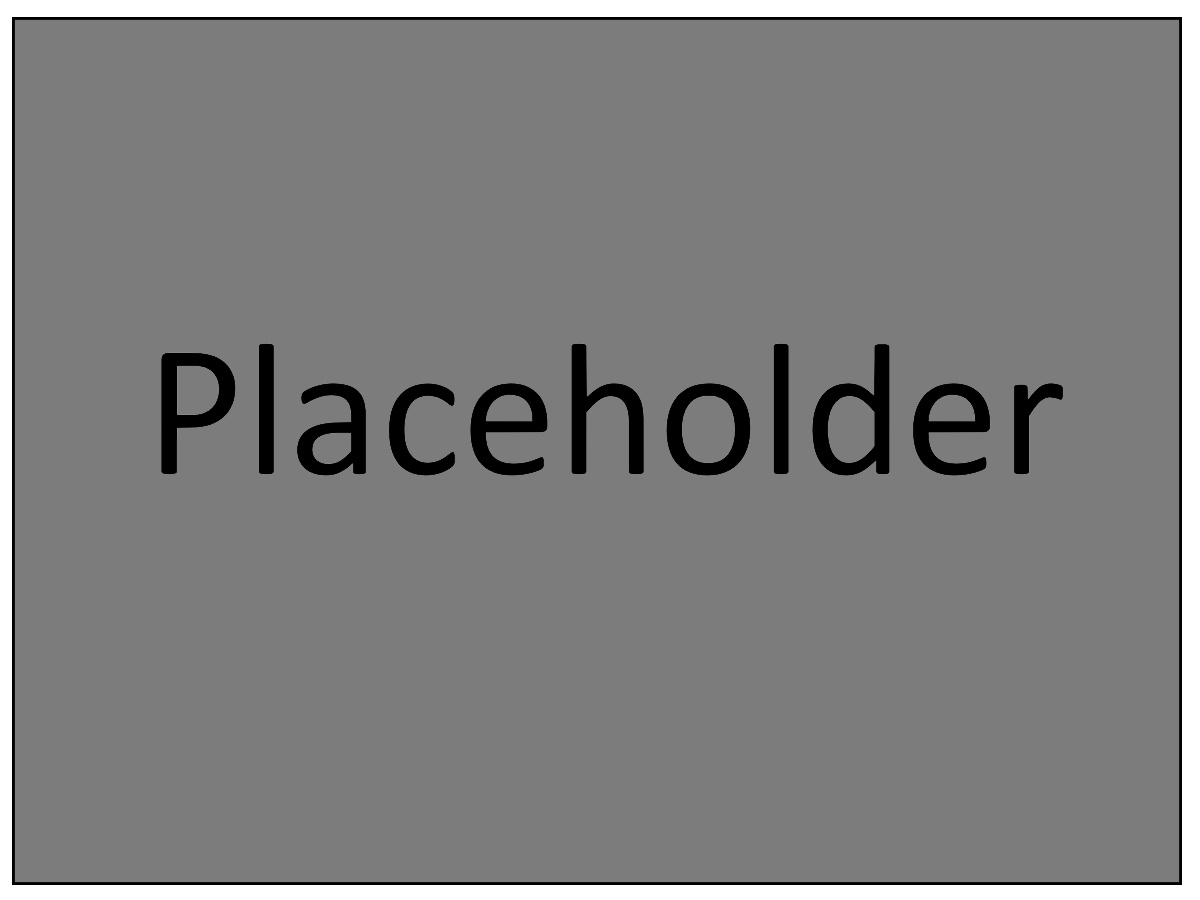
\includegraphics[height=3cm]{figures/placeholder.jpg}
    \caption[Placeholder graphics]{A graphic acting as a placeholder for actual images}
    \label{fig:placeholder}
\end{figure}

\section{Main Part 2}\label{sec:main-part-2}
\Blindtext[13]
\cite{googleSearch2024}


\chapter{Summary}\label{ch:summary}

\Blindtext[5]


\backmatter
\pagenumbering{Roman}

\appendix

{\let\clearpage\relax \chapter{Appendix}\label{ch:appendix}}

\appendixsection{Supplemental Material}

\lstinputlisting[language=Python, basicstyle=\footnotesize\ttfamily, caption={[Example hello world script]An example script printing out \enquote{Hello, World!} not using \texttt{\gls{numpy}}}, captionpos=b, label={code:hello-world}]{listings/hello-world.py}

\Blindtext[3]


\bibliographystyle{IEEEtran}
\bibliography{refs}

\printglossary[type=main]

\printglossary[type=libs]

\end{document}
